\documentclass{beamer}
\usepackage{fancyvrb}

\usecolortheme{rose}
\usefonttheme{structurebold}
\setbeamercovered{again covered=\opaqueness<1->{50}}

\title[hsms]{Introduction to Hardware Security Modules}
\author{Joseph Birr-Pixton\\
@jpixton\\
http://jbp.io/}
\date{}

\begin{document}

\frame{\titlepage}

\frame
{
  \frametitle{Intro to HSMs}

  \begin{enumerate}
    \item<1> What's a HSM?
    \item<2> Who buys them?
    \item<3> What do they do?
    \item<4> And not do?
    \item<5> `Fun' with standards
  \end{enumerate}
}

\frame
{
  \frametitle{Introduction}
  Who the hell am I?

  \begin{itemize}
    \item<1->{Wrote software and firmware for nCipher 2005-2012.}
    \item<2->{nCipher acquired by Thales 2008.}
  \end{itemize}
}

\frame
{
  \frametitle{WTF is an HSM?}

  \uncover<1->{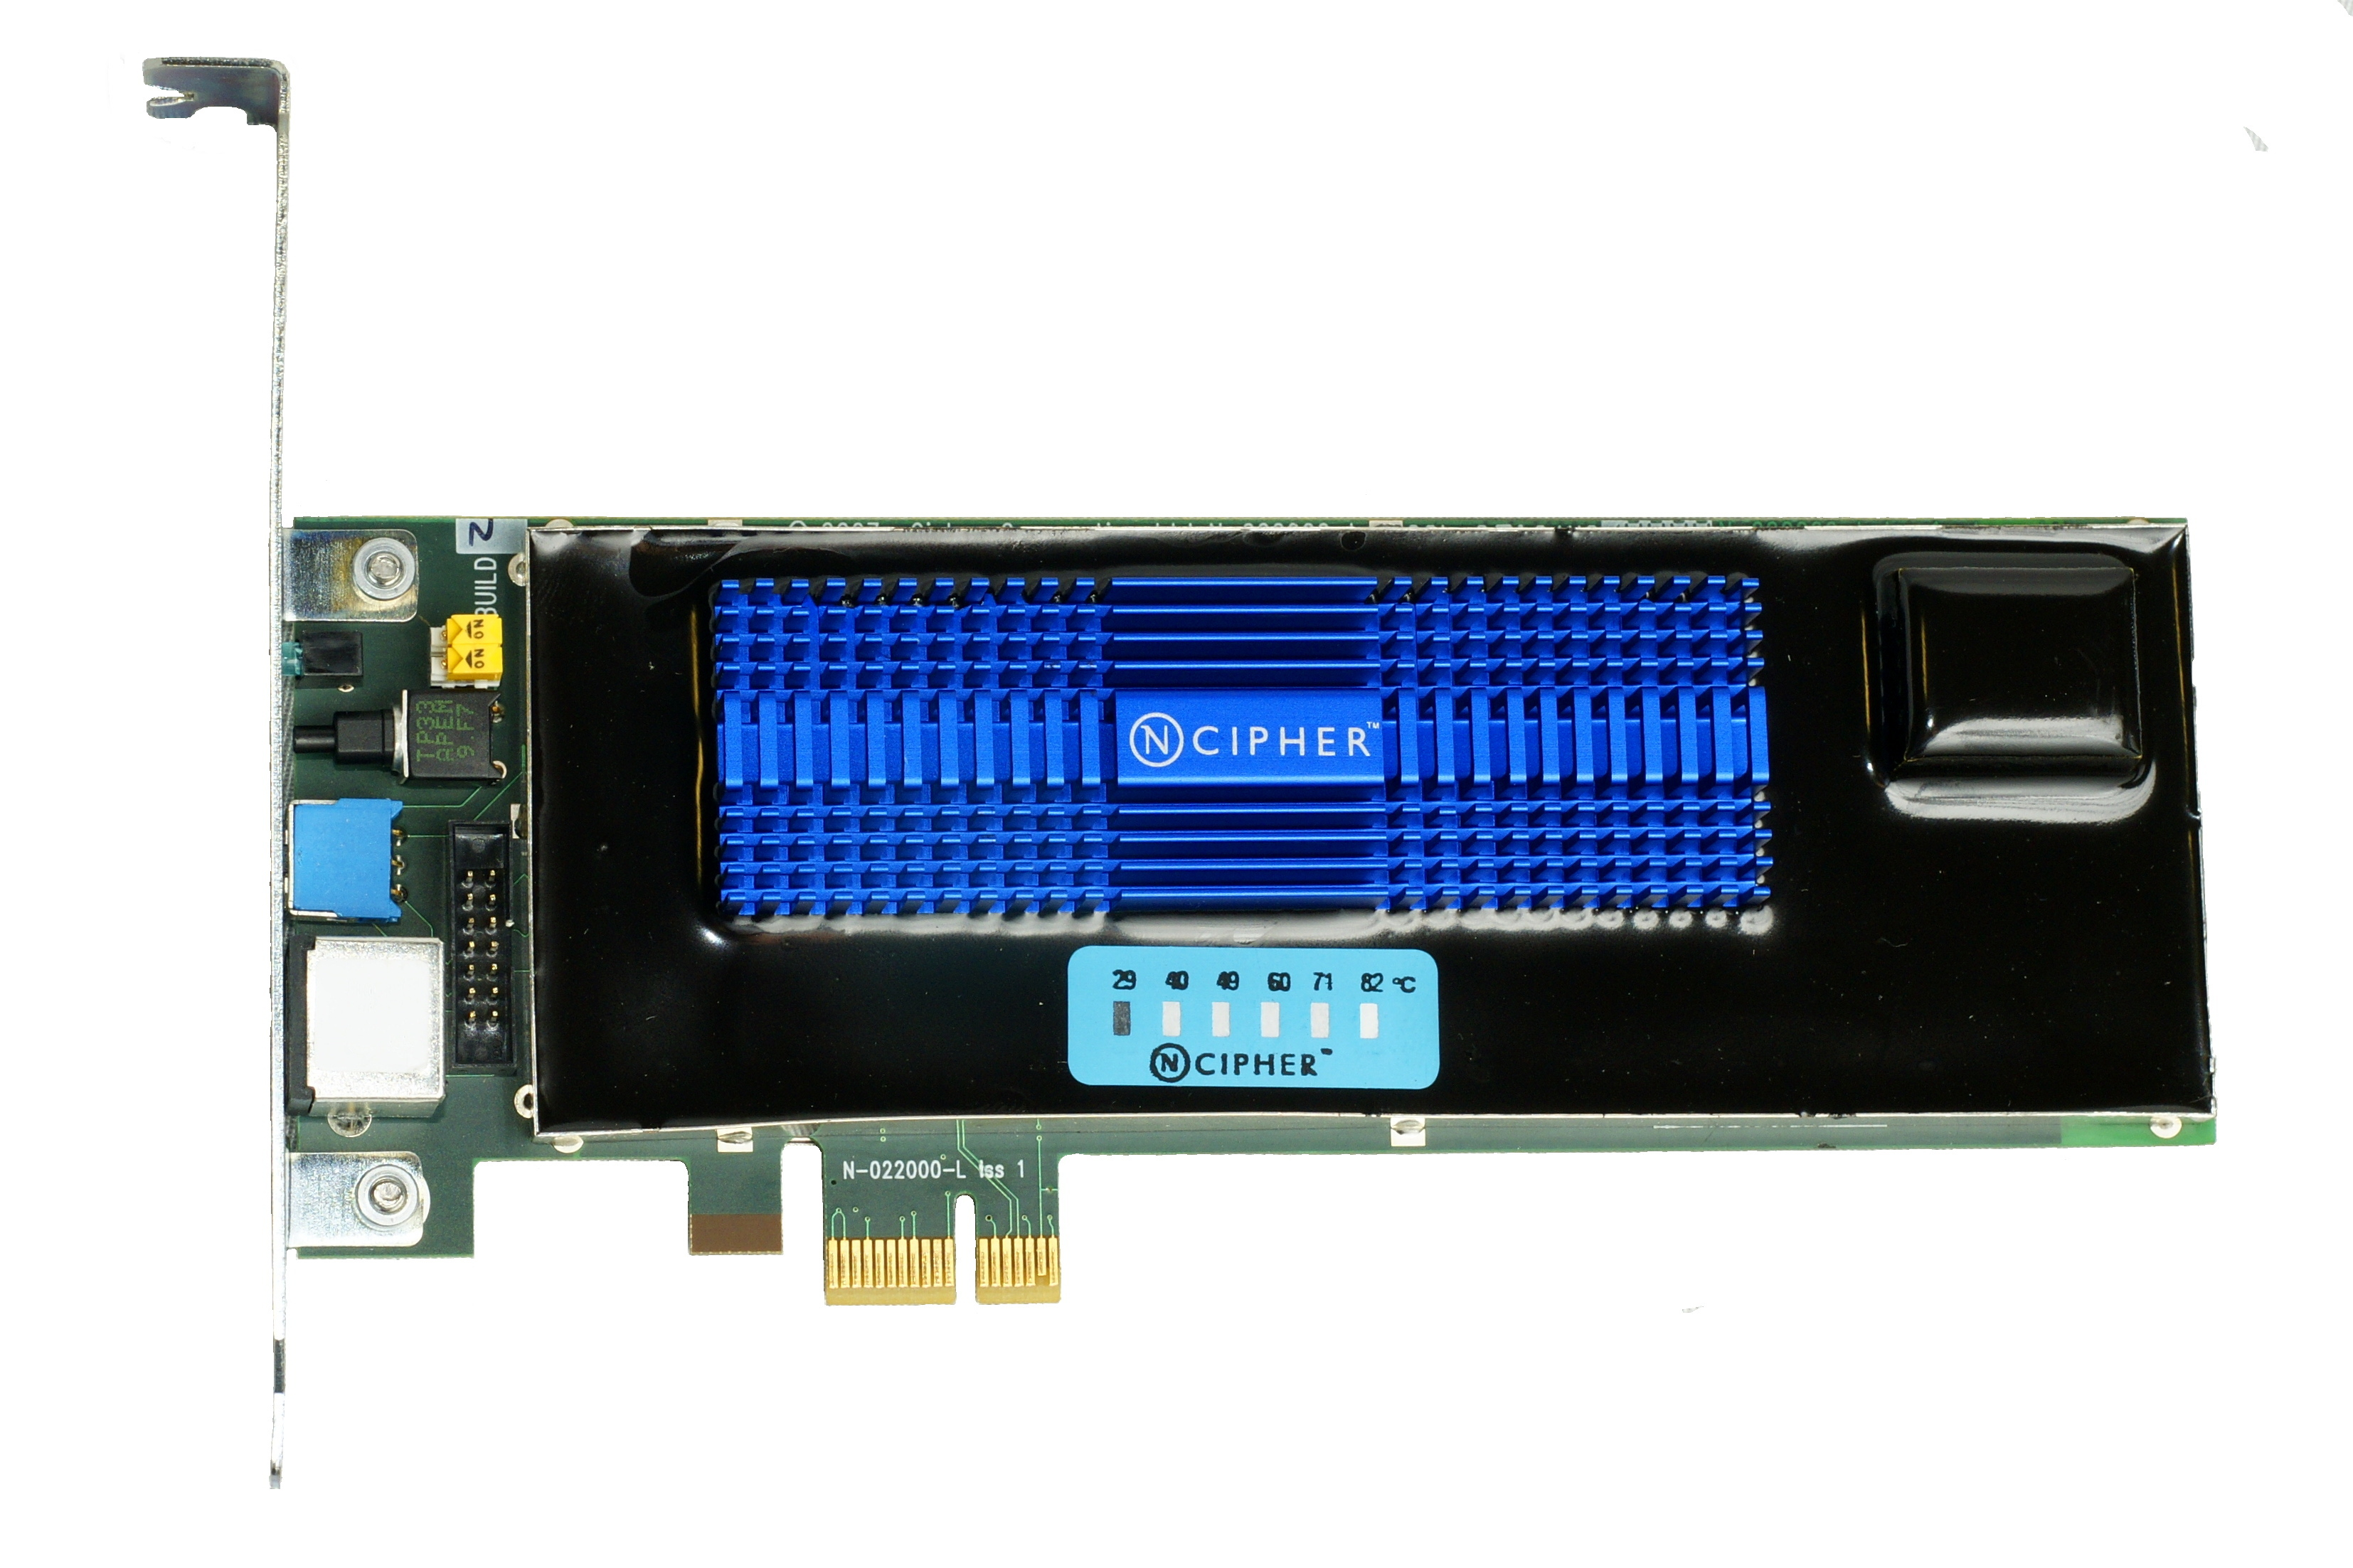
\includegraphics[width=1.0\textwidth]{imgs/NCipher_nShield_F3_Hardware_Security_Module.jpg}}
}

\frame
{
  \frametitle{WTF is an HSM?}

  \begin{itemize}
  \item<1-> Usually built from general purpose CPU, RAM, non-volatile storage.
  \item<2-> Often with a commercial or custom crypto accelerator.
  \item<3-> A communications path to talk to the thing (PCI, PCIe, ethernet, USB, etc.)
  \item<4-> Hardware typically has physical protection:
    \begin{itemize}
    \item<5-> \emph{Tamper evident} hardware usually potted in epoxy-based compound.
    \item<6-> \emph{Tamper reactive} hardware usually enclosed in tamper sensing membrane, with active response circuitry within.
    \end{itemize}
  \item<7-> Tamper reactive hardware rare in HSMs; more common in things in adversarial environments like payments terminals.
  \end{itemize}
}

\frame
{
  \frametitle{Who buys them?}

  Payments HSMs:
  
  \begin{itemize}
    \item<1-> Single-purpose.
    \item<2-> Implement various financial crypto standards, but rarely anything else.
    \item<3-> Sold entirely to banks, payments processors, financial services.
  \end{itemize}

  \uncover<4->{General purpose HSMs:}

  \begin{itemize}
    \item<4-> Standard, sometimes modern crypto.
    \item<5-> Integration with standard APIs (OpenSSL, PKCS\#11, Microsoft CNG, etc.)
    \item<6-> Sold to governments and industry.
  \end{itemize}
}

\frame
{
  \frametitle{What do they do?}

  \begin{itemize}
    \item<1-> Well, crypto...
    \item<2-> But mainly: key management.  \uncover<3->{Like:}
      \begin{itemize}
        \item<3-> Dual control: 'any 3 of these 5 people can use the key'
        \item<4-> Complex key policies: 'this RSA key can only decrypt using OAEP'
        \item<5-> Providing a decent way to back up key material
      \end{itemize}
  \end{itemize}
}

\frame
{
  \frametitle{What don't they do?}

  \begin{itemize}
    \item<1-> HSMs don't know best; they do what they're told
    \begin{itemize}
      \item<2-> Compromised hosts are a common overall problem with systems containing HSMs.
                
      \uncover<3->{
\includegraphics[width=0.5\textwidth]{imgs/diginotarlogo.png}}

      \item<4-> Understanding and expressing the policy you want is an ongoing problem.
    \end{itemize}

    \item<5-> Don't do crypto any quicker (in general) than software running on a modern CPU.
    \item<6-> Don't fix a system using rubbish crypto (RC4, unauthenticated block cipher modes, RSA PKCS\#1 encryption, MD5/SHA1 signatures, ...)
  \end{itemize}
}

\frame
{
  \frametitle{`Fun' with standards}

  \begin{itemize}
    \item<1-> Most (75\%?) of custom is driven by `compliance.'
    \item<2-> Other customers are eager/paranoid security folks.
  \end{itemize}

  \begin{itemize}
    \item<3-> FIPS 140-2 is the main standard for HSMs (and software crypto modules).
    \item<4-> Implemented crypto standards come from NIST, IEEE, ANSI, KISA, etc. usually at request of customers.
      \begin{itemize}
        \item<5-> Some requests are `interesting.'
      \end{itemize}
  \end{itemize}
}

\frame
{
  \frametitle{Fin}
  Questions?

  \vspace{5em}

  Twitter: @jpixton
  
  Web: http://jbp.io/
}

\end{document}
